\documentclass[12pt]{article}
\usepackage[margin=1in]{geometry}
\usepackage{amsmath}
\usepackage{amssymb}
\usepackage{graphicx}
\usepackage{tikz}
\usetikzlibrary{arrows.meta, positioning, shapes.geometric, calc}
\usepackage{booktabs}
\usepackage{hyperref}
\usepackage[capitalise]{cleveref}
\usepackage{microtype}
\usepackage{fancyvrb}
\usepackage{parskip}          % no paragraph indent; vertical space between paragraphs

% Placeholder for figures not yet drawn
\newcommand{\figplaceholder}[2][3in]{%
  \begin{center}
  \fbox{\parbox{#1}{\centering\vspace{0.5in}\textit{[Figure: #2]}\vspace{0.5in}}}
  \end{center}
}

\title{PID Control: From Analysis to Practice\\[0.5em]
\large ME 2801 Supplementary Article}
\author{}
\date{}

\begin{document}
\maketitle
\tableofcontents
\newpage

% ===========================================================================
\section{Introduction}
\label{sec:intro}
% ===========================================================================

Every controlled system faces the same fundamental problem: you want an output
to follow a desired value, but the plant doesn't do what you ask unless you
continuously correct it.  A ship asked to hold a heading will drift off course
in wind and current.  A vessel asked to cruise at a fixed speed will slow down
as it climbs a river current.  Open-loop control --- computing a fixed input
and hoping for the best --- only works when your model is perfect and
disturbances don't exist.

Feedback control addresses this by closing the loop: measure the output,
compare it to the desired value, and use that \emph{error} to drive the input.
The question then becomes: exactly what do you do with the error?  The answer
that has dominated engineering practice for nearly a century is
\emph{proportional-integral-derivative (PID) control}.

PID is the workhorse of industrial and marine control systems.  The autopilot
keeping a surface ship on course, the speed governor on a submarine's propulsion
system, the altitude-hold function on an aircraft's flight control computer ---
these all rely on variants of the same three-term structure.  Its staying power
comes from three practical virtues:
\begin{enumerate}
\item Simple to understand and implement
\item Can work without a detailed mathematical model of the plant --- although a
  model can be a huge help in understanding.
\item The three parameters can be tuned in the field by engineers who
  understand what each one does.
\end{enumerate}

That last point --- understanding what each parameter \emph{does} --- is what
this article is about.  Most treatments of PID present the equations and then
move quickly to formulas for choosing gains.  This article takes the opposite
approach: we will spend most of our time building physical intuition for each
term before touching a tuning method.  The goal is that when you look at a
poorly performing response, you can diagnose what is wrong and know which
knob to turn.

\subsection*{Running Examples}

Throughout this article we will use two running examples drawn directly from
the USV lab.

\begin{figure}[htbp]
\centering
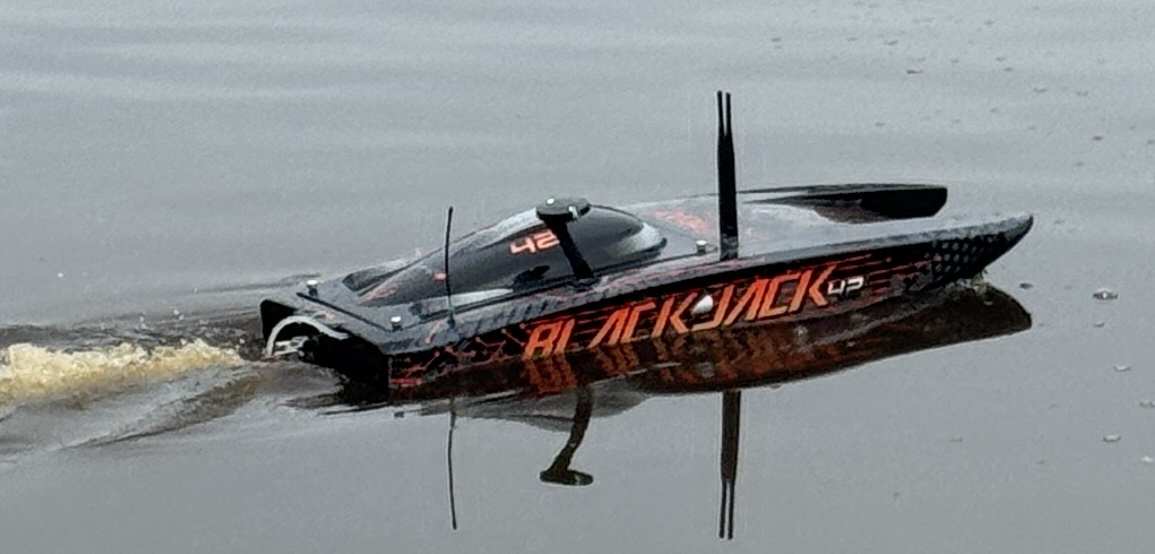
\includegraphics[width=0.7\textwidth]{images/usv_nps.jpg}
\caption{The USV used in the lab.}
\label{fig:usv}
\end{figure}

\textbf{Surge (speed) control.}
The USV's forward speed response to throttle can be approximated by a
first-order transfer function.  The objective is to hold a desired speed in the presence of disturbances like current and wind --- it is a
\emph{constant-setpoint tracking problem}, the simplest and most common control
scenario.

\textbf{Heading control.}
The USV's yaw-rate response to rudder is also first-order, but the performance
metric we care about is \emph{heading} (yaw angle), which is the integral of
yaw rate.  This mismatch between the plant output and the performance metric
turns out to be the key motivation for \emph{cascade control}: an inner loop
that regulates yaw rate quickly, wrapped inside an outer loop that uses that
fast inner response to achieve precise heading.  This is also the architecture
used by ArduRover.


% ===========================================================================
\section{The PID Controller}
\label{sec:pid}
% ===========================================================================

\subsection{Intuition Before Math}

The PID controller computes a corrective input from three components of the
error $e(t) = r(t) - y(t)$, where $r(t)$ is the reference (also called
the \emph{command} or \emph{setpoint}) and $y(t)$ is the measured output.

\begin{description}
  \item[Proportional ($K_P$)] React to the current error.  If the vessel is
    2\,m/s below target speed, apply a corrective throttle proportional to
    that gap.  Larger error, larger correction.
  \item[Integral ($K_I$)] Adapt to the history of error.  If a river current
    has been persistently slowing the vessel, the integrator builds up a
    sustained correction over time to compensate. 
  \item[Derivative ($K_D$)] Anticipate the trend.  If the speed error is
    shrinking rapidly --- the vessel is closing in on its target --- the
    derivative term begins reducing the throttle command before the speed
    overshoots.
\end{description}

A useful analogy is a driver trying to hold a fixed highway speed.  The P term
is how firmly they press the pedal in proportion to how far off-speed they are.
The I term represents what the driver has learned about the road grade and
headwind --- accumulated experience that shows up as a steady baseline pressure
on the pedal.  The D term is the instinctive easing-off as the speedometer
needle swings rapidly toward the target.

\subsection{Transfer Function Form}

The time-domain PID law is:
\begin{equation}
  u(t) = K_P\, e(t) \;+\; K_I \int_0^t e(\tau)\,d\tau \;+\; K_D\, \dot{e}(t)
  \label{eq:pid_time}
\end{equation}

Taking the Laplace transform gives the controller transfer function:
\begin{equation}
  C(s) = K_P + \frac{K_I}{s} + K_D s = \frac{K_D s^2 + K_P s + K_I}{s}
  \label{eq:pid_tf}
\end{equation}

Two features are worth noting.  First, there is one pole at $s = 0$: the
integrator.  We will see in \cref{sec:integral} exactly why this eliminates
steady-state error.  Second, there are two zeros, at the roots of
$K_D s^2 + K_P s + K_I = 0$.  The designer places these anywhere in the
complex plane by choosing $K_P$, $K_I$, and $K_D$ --- significant freedom to
shape the closed-loop response.

Note that $K_D s$ grows without bound as $s \to \infty$.  This means the ideal
PID transfer function is \emph{improper} and cannot be implemented exactly in
hardware or software.  In practice, the D term always includes a high-frequency
limit; we will address this in \cref{sec:practical}.

\subsection{Closed-Loop Transfer Function}

\begin{figure}[htbp]
\centering
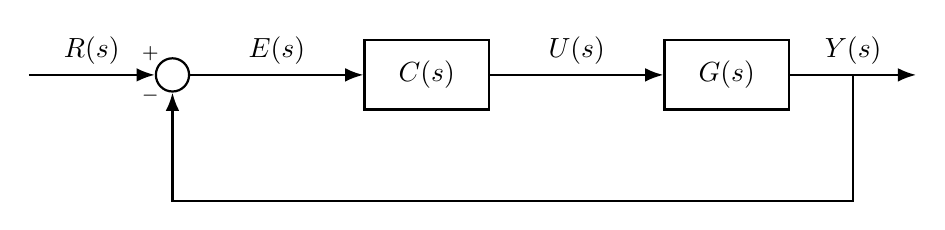
\begin{tikzpicture}[
  >=Latex, thick,
  block/.style = {draw, rectangle, minimum height=2.5em, minimum width=4.5em},
  sum/.style   = {draw, circle, inner sep=0pt, minimum size=1.2em},
]
  \node[coordinate]                   (rin)  {};
  \node[sum,   right=1.6cm of rin]    (sum)  {};
  \node[block, right=2.2cm of sum]    (C)    {$C(s)$};
  \node[block, right=2.2cm of C]      (G)    {$G(s)$};
  \node[coordinate, right=1.6cm of G] (yout) {};

  % Signs at summing junction
  \node[font=\scriptsize, inner sep=0pt, anchor=south east] at (sum.north west) {$+$};
  \node[font=\scriptsize, inner sep=0pt, anchor=north east] at (sum.south west) {$-$};

  % Forward path
  \draw[->] (rin)  -- node[above]{$R(s)$}  (sum);
  \draw[->] (sum)  -- node[above]{$E(s)$}  (C);
  \draw[->] (C)    -- node[above]{$U(s)$}  (G);
  \draw[->] (G)    -- node[above]{$Y(s)$}  (yout);

  % Feedback path: down from midpoint of output wire, left, up into sum
  \coordinate (fbk) at ($(G.east)!0.5!(yout)$);
  \draw[->] (fbk) -- ++(0,-1.6) -| (sum.south);
\end{tikzpicture}
\caption{Standard unity-feedback control loop.}
\label{fig:unity_feedback}
\end{figure}

For the loop in \cref{fig:unity_feedback}, the output is $Y = C(s)G(s)E$ and
the error is $E = R - Y$.  Substituting:
\[
  Y = C(s)G(s)\bigl(R - Y\bigr)
  \implies Y\bigl(1 + C(s)G(s)\bigr) = C(s)G(s)\,R
\]
so the closed-loop transfer function is:
\begin{equation}
  T(s) = \frac{Y(s)}{R(s)} = \frac{C(s)G(s)}{1 + C(s)G(s)}
  \label{eq:cltf}
\end{equation}

The order of the closed-loop equals the number of poles in $C(s)G(s)$.  A PID
controller adds one pole (the integrator at $s=0$) to whatever poles the plant
already has.  For our first-order surge plant, the closed-loop will be
second-order once integral action is included.

The zeros of $C(s)$ also appear as zeros of $T(s)$.  Controller zeros speed up
the transient response and can introduce overshoot --- something to keep in mind
as we add integral and derivative terms.


% ===========================================================================
\section{Proportional Control on a First-Order Plant}
\label{sec:pcontrol}
% ===========================================================================

\subsection{The USV Surge Model}

Linear analysis of the surge dynamics (forward speed vs.\ throttle) yields a
first-order transfer function:
\begin{equation}
  G(s) = \frac{K}{\tau s + 1}
  \label{eq:surge_plant}
\end{equation}
where $K$ is the steady-state speed per unit throttle (m/s per unit effort)
and $\tau$ is the time constant set by the balance of inertia and drag.
Throttle is normalized to $\pm 1$, with $+1$ being full forward effort and
$-1$ full reverse.

\subsection{Closed-Loop with P Only}

With a pure proportional controller $C(s) = K_P$, the open-loop transfer
function is $C(s)G(s) = K_P K/(\tau s + 1)$.  Substituting into
\cref{eq:cltf}:
\begin{equation}
  T_P(s) = \frac{K_P K/(\tau s+1)}{1 + K_P K/(\tau s+1)}
          = \frac{K_P K}{\tau s + 1 + K_P K}
          = \frac{K_\infty}{\tau_\mathrm{cl}\,s + 1}
  \label{eq:cl_p}
\end{equation}
where:
\begin{equation}
  K_\infty = \frac{K_P K}{1 + K_P K}, \qquad
  \tau_\mathrm{cl} = \frac{\tau}{1 + K_P K}
  \label{eq:p_params}
\end{equation}

The closed-loop is still first-order --- proportional control does not change
the system order.  But compared to the open-loop plant, two things have
changed: the time constant is smaller (faster response) and the DC gain is
less than one.

The DC gain of the closed-loop system, $K_\infty$ is less than one, which is the root of the problem.  For a unit step in
desired speed, the steady-state output is $K_\infty$, so the
\emph{steady-state error} is:
\begin{equation}
  e_{ss} = 1 - K_\infty = \frac{1}{1 + K_P K}
  \label{eq:p_error}
\end{equation}

\begin{figure}[htbp]
\centering

\includegraphics[width=\linewidth]{images/p_step.pdf}
\caption{Step response of the P-controlled surge plant for increasing
  proportional gain.  Higher gain improves speed and reduces error, but steady-state
  error persists regardless.}
\label{fig:p_step}
\end{figure}

\Cref{fig:p_step} illustrates the trade-off: increasing $K_P$ makes the
response faster and reduces steady-state error, but the error never reaches
zero.  To eliminate it entirely, we need a different kind of controller action.

One more note: a first-order plant with proportional-only control cannot
become unstable.  The closed-loop pole is at $s = -(1+K_P K)/\tau$, which
is always in the left half-plane for positive gains.  The only cost of
increasing $K_P$ is noisier, jerkier actuator behavior --- not instability.
This will not be true once the plant order increases or a second loop is closed.


% ===========================================================================
\section{Adding Integral Action}
\label{sec:integral}
% ===========================================================================

\subsection{Why Integral Eliminates Steady-State Error}

The intuitive argument is straightforward.  At steady state, all signals are
constant and $\dot{u} = 0$.  The integral term contributes
$K_I \int e\,dt$ to the control output.  For this contribution to be
constant, its integrand must be zero --- meaning $e = 0$.  Any nonzero
steady-state error would keep the integrator growing, contradicting the
assumption of steady state.  Therefore, if the loop is stable, the
steady-state error to a step reference must be zero.

More formally: the PI controller has a pole at $s=0$, making the open-loop
transfer function Type 1.  By the final value theorem, a Type 1 loop tracks
step references with zero steady-state error.

\subsection{PI on the Surge Plant}

With $C(s) = K_P + K_I/s = (K_P s + K_I)/s$, the open-loop transfer function
is:
\[
  C(s)G(s) = \frac{K(K_P s + K_I)}{s(\tau s + 1)}
\]

The closed-loop transfer function is:
\begin{equation}
  T_{PI}(s) = \frac{K(K_P s + K_I)}{\tau s^2 + (1 + KK_P)s + KK_I}
  \label{eq:cl_pi}
\end{equation}

The denominator --- the \emph{characteristic polynomial} --- is now
second-order.  Writing it in standard form $s^2 + 2\zeta\omega_n s + \omega_n^2$
(after dividing by $\tau$):

\begin{equation}
  \omega_n = \sqrt{\frac{KK_I}{\tau}}, \qquad
  \zeta = \frac{1 + KK_P}{2\sqrt{\tau K K_I}}
  \label{eq:pi_params}
\end{equation}

These two expressions directly guide design:
\begin{itemize}
  \item $K_I$ controls the natural frequency $\omega_n$.  Choose $K_I$ to
    set the desired speed of response: $K_I = \omega_n^2\tau/K$.
  \item $K_P$ primarily controls the damping ratio $\zeta$ (through the
    $(1+KK_P)$ numerator term).  Once $K_I$ is fixed, choose $K_P$ to
    target a desired $\zeta$: $K_P = (2\zeta\omega_n\tau - 1)/K$.
  \item For $\zeta < 1/\sqrt{2} \approx 0.707$, the response will overshoot.
    For $\zeta > 1$, it will be overdamped.  A common target is
    $\zeta \approx 0.707$, which gives near-critical damping with no
    significant overshoot.
\end{itemize}

The closed-loop also has a zero at $s = -K_I/K_P$, inherited from the PI
controller.  This zero does not affect the stability (poles determine that),
but it does pull the step response slightly faster and may add a small amount
of overshoot beyond what the poles alone would predict.  The effect is larger
when the zero is close to the imaginary axis --- that is, when $K_I/K_P$ is
small.  This reinforces a useful design heuristic: add integral action only
when needed to eliminate steady-state error, and keep $K_I$ small relative
to $K_P$.  A large $K_I$ pulls the zero close to the origin, amplifies the
overshoot contribution of the zero, and risks the windup problem described
below.

\begin{figure}[htbp]
\centering

\includegraphics[width=\linewidth]{images/pi_compare.pdf}
\caption{Comparison of P-only and PI step responses on the surge plant.}
\label{fig:pi_compare}
\end{figure}

\subsection{Integral Windup}

The integrator is powerful, but it has a failure mode.  When the actuator
saturates --- throttle clipped at its maximum value --- the plant input is no
longer following the controller output.  The error persists, the integrator
keeps growing, and by the time the plant output finally approaches the setpoint,
the integrator has accumulated a large value that drives a large overshoot
before it can unwind.  This is \emph{integral windup}.

A concrete scenario: the USV is commanded to accelerate from rest to full
cruise speed.  The throttle saturates at its maximum for the entire ramp-up.
During this time the error is large and positive, and the integrator accumulates
a large value.  When the speed finally reaches the setpoint, the controller
output is still large because of the accumulated integral, pushing the throttle
above what is needed and causing the vessel to overshoot before the integrator
can recover.  \Cref{sec:practical} addresses fixes.

\begin{figure}[htbp]
\centering

\includegraphics[width=\linewidth]{images/windup.pdf}
\caption{Integral windup: the area accumulated under $e(t)$ during saturation
  must be ``paid back,'' causing overshoot and slow recovery once the output
  leaves saturation.}
\label{fig:windup}
\end{figure}

% ===========================================================================
\section{Derivative Action}
\label{sec:derivative}
% ===========================================================================

\subsection{Derivative as Anticipation}

The derivative term $K_D \, \dot{e}(t)$ responds to the \emph{rate of change}
of error, not its current value.  When the error is decreasing rapidly --- the
output is converging on the setpoint quickly --- the derivative term provides
a braking action that reduces overshoot.  The analogy is a shock absorber:
it resists velocity, not displacement.

Unlike the proportional term, which reacts to where you are, and the integral,
which reacts to where you have been, the derivative reacts to where you are
going.

\subsection{PID on the Surge Plant}

Adding the derivative term to PI gives the full PID controller.  The
characteristic polynomial of the closed-loop becomes:
\begin{align}
  \Delta(s) &= s(\tau s + 1) + K(K_D s^2 + K_P s + K_I) \nonumber\\
            &= (\tau + KK_D)\,s^2 + (1 + KK_P)\,s + KK_I
  \label{eq:pid_charpoly}
\end{align}

Comparing to the PI case \eqref{eq:cl_pi}, the derivative term increases the
coefficient of $s^2$ from $\tau$ to $\tau + KK_D$.  This has two effects on
the natural frequency and damping ratio:
\begin{equation}
  \omega_n = \sqrt{\frac{KK_I}{\tau + KK_D}}, \qquad
  \zeta = \frac{1 + KK_P}{2\sqrt{(\tau + KK_D)KK_I}}
  \label{eq:pid_params}
\end{equation}

The D term \emph{lowers} $\omega_n$ and \emph{raises} $\zeta$.  In physical
terms: derivative action slows the natural frequency slightly while adding
damping.  If a PI-controlled system is too oscillatory (low $\zeta$), adding
$K_D$ is one way to fix it.

On a first-order plant, however, $K_P$ already provides a path to increasing
$\zeta$ (via the $1+KK_P$ numerator term in $\zeta$).  The derivative term
provides an additional handle but is not strictly necessary.  For second-order
plants, where the P term alone cannot independently set both $\omega_n$ and
$\zeta$, derivative action is far more valuable.  This is the general rule: D
matters most when the plant itself has dynamics that limit the damping
achievable with P and I alone.

\begin{figure}[htbp]
\centering

\includegraphics[width=\linewidth]{images/d_noise.pdf}
\caption{Sensor noise amplification by the derivative term.  Small
  fluctuations in the measurement are amplified, becoming large spikes in $\dot{u}$.}
\label{fig:d_noise}
\end{figure}

\subsection{The Noise Problem}

The ideal D term $K_D s$ has a transfer function whose gain grows without
bound at high frequencies.  Sensor noise consists of rapid, small fluctuations.
An unfiltered D term amplifies these into large, noisy actuator commands --- a
propeller being driven in rapid small oscillations around its mean command.
This issue, the \emph{dirty derivative}, is why pure derivative is never implemented in practice, and why the D term is often omitted entirely in noisy systems.

The solution is discussed in \cref{sec:practical}: add a first-order low-pass filter to
the D term that caps its gain at high frequencies while preserving its
damping effect at the frequencies of interest.


% ===========================================================================
\section{Cascade Control for Heading}
\label{sec:cascade}
% ===========================================================================

\subsection{The Problem with a Single Heading Loop}

The USV's yaw dynamics are well-modeled by a first-order relationship between
rudder input and yaw rate $\dot\psi$:
\begin{equation}
  G_r(s) = \frac{K_r}{\tau_r s + 1}
  \label{eq:yaw_rate_plant}
\end{equation}

The performance objective, however, is heading $\psi$ --- the integral of yaw
rate.  Heading is related to rudder by:
\begin{equation}
  G_\psi(s) = \frac{G_r(s)}{s} = \frac{K_r}{s(\tau_r s + 1)}
  \label{eq:heading_plant}
\end{equation}

This is a second-order, Type 1 plant (one integrator from the kinematics).
Applying a simple proportional heading controller $C_\psi(s) = K_\psi$:
\[
  C_\psi G_\psi = \frac{K_\psi K_r}{s(\tau_r s + 1)}
\]
\begin{equation}
  \omega_n = \sqrt{\frac{K_\psi K_r}{\tau_r}}, \qquad
  \zeta = \frac{1}{2\sqrt{K_\psi K_r \tau_r}}
  \label{eq:heading_p}
\end{equation}

Notice that $\zeta \propto 1/\sqrt{K_\psi}$.  Increasing the gain to get a
faster heading response simultaneously reduces damping.  With only one
parameter ($K_\psi$), the designer cannot independently choose both speed and
damping --- a fundamental limitation of the single-loop approach.

\subsection{The Cascade Architecture}

Cascade (inner/outer loop) control resolves this by splitting the heading
problem into two simpler problems:

\begin{enumerate}
  \item \textbf{Inner loop} (yaw rate): a fast controller $C_r(s)$ tracks a
    commanded yaw rate $\dot\psi_\mathrm{des}$.  The plant is the first-order
    $G_r(s)$ --- straightforward to control well with PI.
  \item \textbf{Outer loop} (heading): a slow controller $C_\psi(s)$
    computes the yaw-rate command based on the heading error.  It ``sees''
    the inner loop as its plant.
\end{enumerate}

\begin{figure}[htbp]
\centering
\resizebox{\linewidth}{!}{%
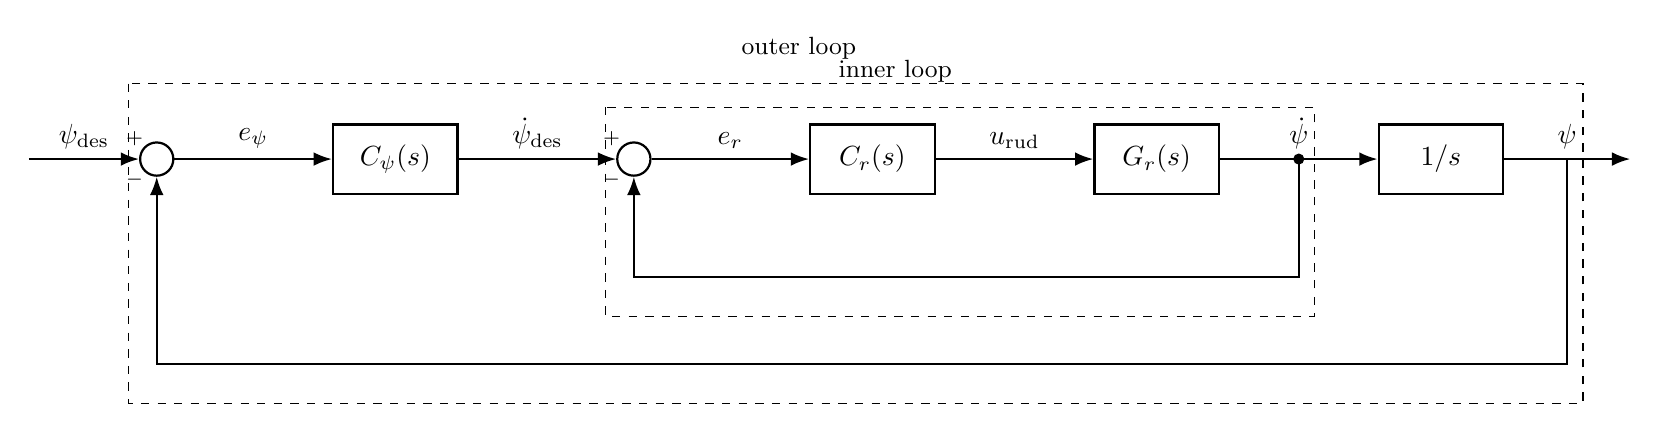
\begin{tikzpicture}[
  >=Latex, thick,
  block/.style = {draw, rectangle, minimum height=2.5em, minimum width=4.5em},
  sum/.style   = {draw, circle, inner sep=0pt, minimum size=1.2em},
]
  % Outer loop nodes
  \node[coordinate]                              (rin)   {};
  \node[sum,   right=1.4cm of rin]               (oes)   {};
  \node[block, right=2.0cm of oes]               (Cpsi)  {$C_\psi(s)$};

  % Inner loop nodes
  \node[sum,   right=2.0cm of Cpsi]              (ies)   {};
  \node[block, right=2.0cm of ies]               (Cr)    {$C_r(s)$};
  \node[block, right=2.0cm of Cr]                (Gr)    {$G_r(s)$};

  % Integrator (yaw rate -> heading)
  \node[block, right=2.0cm of Gr]                (Int)   {$1/s$};
  \node[coordinate, right=1.6cm of Int]          (yout)  {};

  % Labels
  \node[font=\scriptsize, inner sep=0pt, anchor=south east] at (oes.north west) {$+$};
  \node[font=\scriptsize, inner sep=0pt, anchor=north east] at (oes.south west) {$-$};
  \node[font=\scriptsize, inner sep=0pt, anchor=south east] at (ies.north west) {$+$};
  \node[font=\scriptsize, inner sep=0pt, anchor=north east] at (ies.south west) {$-$};

  % Forward path
  \draw[->] (rin)  -- node[above]{$\psi_\mathrm{des}$}   (oes);
  \draw[->] (oes)  -- node[above]{$e_\psi$}               (Cpsi);
  \draw[->] (Cpsi) -- node[above]{$\dot\psi_\mathrm{des}$}(ies);
  \draw[->] (ies)  -- node[above]{$e_r$}                  (Cr);
  \draw[->] (Cr)   -- node[above]{$u_\mathrm{rud}$}       (Gr);
  \draw[->] (Gr)   -- node[above]{$\dot\psi$}             (Int);
  \draw[->] (Int)  -- node[above]{$\psi$}                 (yout);

  % Inner feedback: branch after Gr, close around yaw rate
  \coordinate (iyfbk) at ($(Gr.east)!0.5!(Int.west)$);
  \fill (iyfbk) circle (2pt);
  \draw[->] (iyfbk) -- ++(0,-1.5) -| (ies.south);

  % Outer feedback: branch after Int, close around heading
  \coordinate (oyfbk) at ($(Int.east)!0.5!(yout)$);
  \draw[->] (oyfbk) -- ++(0,-2.6) -| (oes.south);

  % Brace annotations for loop boundaries
  \draw[dashed, thin]
      ($(ies.north west)+(-0.2,0.5)$) rectangle ($(iyfbk)+(0.2,-2.0)$);
  \node[above, font=\small] at ($(ies.north)!0.5!(Gr.north)+(0,0.5)$)
      {inner loop};

  \draw[dashed, thin]
      ($(oes.north west)+(-0.2,0.8)$) rectangle ($(oyfbk)+(0.2,-3.1)$);
  \node[above, font=\small] at ($(oes.north)!0.5!(Int.north)+(0,0.8)$)
      {outer loop};
\end{tikzpicture}}
\caption{Cascade control structure for heading.  The inner loop regulates
  yaw rate; the outer loop regulates heading by commanding a desired yaw rate.}
\label{fig:cascade}
\end{figure}

The fundamental design rule is: \textbf{the inner loop must respond
significantly faster than the outer loop.}  In terms of step response, this
means the inner loop's closed-loop time constant $\tau_\mathrm{cl}$ should
be at least 5 times smaller than the outer loop's desired response time.
Put differently: if the vehicle should reach a commanded heading in roughly
$T$ seconds, the yaw-rate loop should reach a commanded yaw rate in roughly
$T/5$ seconds or less.  If the inner loop is slow, it distorts the signals
the outer loop is trying to control and the approximation in the next section
breaks down.

\subsection{Quantitative Analysis}

Suppose the inner yaw-rate loop is well-tuned and its closed-loop transfer
function $T_{\mathrm{inner}}(s)$, approximates a first-order response:
\begin{equation}
  T_{\mathrm{inner}}(s) = \frac{\dot\Psi(s)}{\dot\Psi_\mathrm{cmd}(s)}
           \approx \frac{1}{\tau_\mathrm{cl}\,s + 1}
  \label{eq:inner_cl}
\end{equation}
where $\tau_\mathrm{cl}$ is small (inner loop is fast).  The outer loop then
sees an effective plant of:
\begin{equation}
  G_\mathrm{eff}(s) = \frac{T_r(s)}{s} \approx \frac{1}{s(\tau_\mathrm{cl}\,s + 1)}
  \label{eq:outer_eff}
\end{equation}

As $\tau_\mathrm{cl} \to 0$, this approaches $1/s$ --- a pure integrator.
With a proportional outer controller $C_\psi(s) = K_\psi$, the outer closed-loop
heading response becomes:
\begin{equation}
  T_\psi(s) \approx \frac{K_\psi/s}{1 + K_\psi/s} = \frac{K_\psi}{s + K_\psi}
  \label{eq:outer_cl_approx}
\end{equation}

This is approximation (which assumes $\tau_{\mathrm{cl}}$ is vanishingly small) is \emph{first-order}, so the closed-loop response is a clean monotone heading response with time
constant $1/K_\psi$ and no overshoot.  The DC gain of \cref{eq:outer_cl_approx}
is unity ($T_\psi(0) = 1$), confirming zero steady-state error for a step
heading command --- the kinematic integrator in the plant makes the outer loop
type-1 even with a proportional-only outer controller.  The single-loop problem of
coupled speed and damping has disappeared: the outer loop simply has one
parameter ($K_\psi$) that sets the heading response speed, and the inner
loop's good damping ensures the approximation holds.

If we remove our assumption of a vanishingly small internal response ($\tau_{\mathrm{cl}} \to 0$) and include the finite inner-loop time constant $\tau_\mathrm{cl}$, the outer
characteristic polynomial is now the quadratic $\tau_\mathrm{cl} s^2 + s + K_\psi$, giving:
\[
  \omega_n = \sqrt{K_\psi/\tau_\mathrm{cl}}, \qquad
  \zeta = \frac{1}{2\sqrt{K_\psi\,\tau_\mathrm{cl}}}
\]

The coupling between $\omega_n$ and $\zeta$ reappears, but with $\tau_\mathrm{cl}$
in place of $\tau_{\mathrm{inner}}$.  Since the inner loop is much faster than the yaw plant
($\tau_\mathrm{cl} \ll \tau_r$), the outer loop natural frequency is much higher
for the same outer gain, and the approximation $T_r \approx 1$ is valid across
the outer loop's operating range.

In ArduRover, the \texttt{ATC\_STR\_RAT\_*} gains configure the inner yaw-rate
loop; a separate navigation controller acts as the outer heading loop.


% ===========================================================================
\section{Feedforward: Using What You Know}
\label{sec:feedforward}
% ===========================================================================

\subsection{Motivation}

Feedback is inherently reactive; it waits for error to develop before
generating a corrective signal.  For a well-designed loop, this delay is
small --- but it is never zero.  If you already know (or can predict) the input
required to achieve a desired output, you can supply that input directly,
without waiting for error to accumulate.  This is \emph{feedforward}.

\begin{figure}[htbp]
\centering
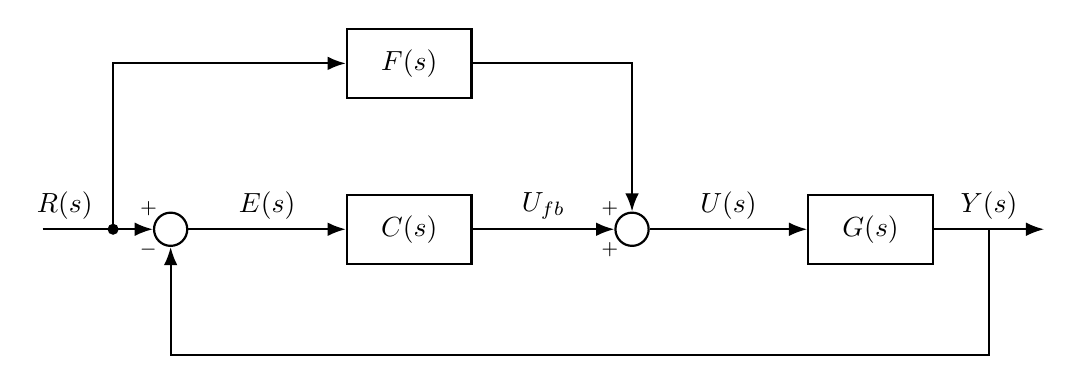
\begin{tikzpicture}[
  >=Latex, thick,
  block/.style = {draw, rectangle, minimum height=2.5em, minimum width=4.5em},
  sum/.style   = {draw, circle, inner sep=0pt, minimum size=1.2em},
]
  \node[coordinate]                    (rin)   {};
  \node[sum,   right=1.4cm of rin]     (esum)  {};
  \node[block, right=2.0cm of esum]    (C)     {$C(s)$};
  \node[sum,   right=1.8cm of C]       (usum)  {};
  \node[block, right=2.0cm of usum]    (G)     {$G(s)$};
  \node[coordinate, right=1.4cm of G]  (yout)  {};

  % FF path above
  \node[block, above=1.2cm of C]       (F)     {$F(s)$};

  \node[font=\scriptsize, inner sep=0pt, anchor=south east] at (esum.north west) {$+$};
  \node[font=\scriptsize, inner sep=0pt, anchor=north east] at (esum.south west) {$-$};
  \node[font=\scriptsize, inner sep=0pt, anchor=south east] at (usum.north west) {$+$};
  \node[font=\scriptsize, inner sep=0pt, anchor=north east] at (usum.south west) {$+$};

  % branch dot on reference wire
  \coordinate (rbranch) at ($(rin)!0.55!(esum)$);
  \draw[->] (rin)     -- node[above, pos=0.2]{$R(s)$}  (esum);
  \fill (rbranch) circle (2pt);

  \draw[->] (rbranch) |- (F);
  \draw[->] (F)       -| (usum);
  \draw[->] (esum)    -- node[above]{$E(s)$}  (C);
  \draw[->] (C)       -- node[above]{$U_{fb}$} (usum);
  \draw[->] (usum)    -- node[above]{$U(s)$}  (G);
  \draw[->] (G)       -- node[above]{$Y(s)$}  (yout);

  \coordinate (fbk) at ($(G.east)!0.5!(yout)$);
  \draw[->] (fbk) -- ++(0,-1.6) -| (esum.south);
\end{tikzpicture}
\caption{Feedforward augments feedback: the FF path provides a predictive
  baseline while feedback corrects residual error.}
\label{fig:ff_block}
\end{figure}

Feedforward and feedback complement each other.  Feedforward handles the
predictable portion of the control effort --- the baseline required to achieve
the desired output in a nominal, disturbance-free environment.  Feedback
handles what feedforward cannot: model error, disturbances, and uncertainty.

\subsection{Two Forms of Feedforward}

\textbf{Operating-point bias} is appropriate when the setpoint is approximately
constant.  Rather than expressing feedforward as a gain, it is parameterized
directly in physical terms: ``at this desired speed, I need this much
throttle.''  The integral term then corrects whatever residual the bias
gets wrong.

\textbf{Proportional (command) feedforward} scales with the reference signal.
For a first-order plant with DC gain $K$, the steady-state input required to
produce output $r$ is simply $u_\mathrm{ff} = r/K$.  Applying this directly
gives immediate response proportional to the command, without waiting for
integral action to build.  This is most useful when the setpoint varies
continuously.

\begin{figure}[htbp]
\centering
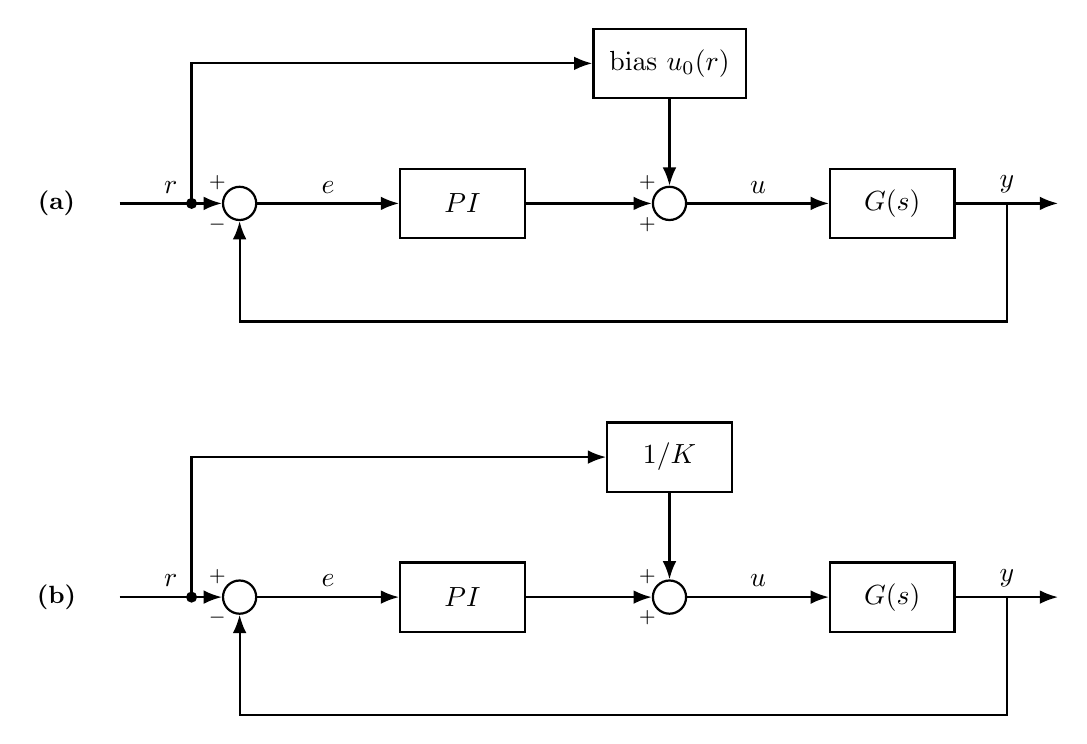
\begin{tikzpicture}[
  >=Latex, thick,
  block/.style = {draw, rectangle, minimum height=2.5em, minimum width=4.5em},
  sum/.style   = {draw, circle, inner sep=0pt, minimum size=1.2em},
]
%--- (a) Operating-point bias (top row) ---
  \node[font=\small\bfseries] at (-0.8,0) {(a)};

  \node[coordinate]                              (arin)  {};
  \node[sum,   right=1.3cm of arin]             (aes)   {};
  \node[block, right=1.8cm of aes]              (aPI)   {$PI$};
  \node[sum,   right=1.6cm of aPI]              (aus)   {};
  \node[block, right=1.8cm of aus]              (aG)    {$G(s)$};
  \node[coordinate, right=1.3cm of aG]          (ayo)   {};

  % bias block above us
  \node[block, above=1.1cm of aus, minimum width=5.5em]
                                                  (abias) {bias $u_0(r)$};

  \node[font=\scriptsize, inner sep=0pt, anchor=south east] at (aes.north west) {$+$};
  \node[font=\scriptsize, inner sep=0pt, anchor=north east] at (aes.south west) {$-$};
  \node[font=\scriptsize, inner sep=0pt, anchor=south east] at (aus.north west) {$+$};
  \node[font=\scriptsize, inner sep=0pt, anchor=north east] at (aus.south west) {$+$};

  \coordinate (arb) at ($(arin)!0.6!(aes)$);
  \draw[->] (arin) -- node[above]{$r$} (aes);
  \fill (arb) circle (2pt);
  \draw[->] (arb) |- (abias);
  \draw[->] (abias) -- (aus.north);
  \draw[->] (aes)  -- node[above]{$e$} (aPI);
  \draw[->] (aPI)  -- (aus);
  \draw[->] (aus)  -- node[above]{$u$} (aG);
  \draw[->] (aG)   -- node[above]{$y$} (ayo);

  \coordinate (afbk) at ($(aG.east)!0.5!(ayo)$);
  \draw[->] (afbk) -- ++(0,-1.5) -| (aes.south);

%--- (b) Proportional FF (bottom row) ---
  \node[font=\small\bfseries] at (-0.8,-5.0) {(b)};

  \node[coordinate, below=5.0cm of arin]        (brin)  {};
  \node[sum,   right=1.3cm of brin]              (bes)   {};
  \node[block, right=1.8cm of bes]               (bPI)   {$PI$};
  \node[sum,   right=1.6cm of bPI]               (bus)   {};
  \node[block, right=1.8cm of bus]               (bG)    {$G(s)$};
  \node[coordinate, right=1.3cm of bG]           (byo)   {};

  % gain block above us
  \node[block, above=1.1cm of bus]               (bFF)   {$1/K$};

  \node[font=\scriptsize, inner sep=0pt, anchor=south east] at (bes.north west) {$+$};
  \node[font=\scriptsize, inner sep=0pt, anchor=north east] at (bes.south west) {$-$};
  \node[font=\scriptsize, inner sep=0pt, anchor=south east] at (bus.north west) {$+$};
  \node[font=\scriptsize, inner sep=0pt, anchor=north east] at (bus.south west) {$+$};

  \coordinate (brb) at ($(brin)!0.6!(bes)$);
  \draw[->] (brin) -- node[above]{$r$} (bes);
  \fill (brb) circle (2pt);
  \draw[->] (brb) |- (bFF);
  \draw[->] (bFF) -- (bus.north);
  \draw[->] (bes)  -- node[above]{$e$} (bPI);
  \draw[->] (bPI)  -- (bus);
  \draw[->] (bus)  -- node[above]{$u$} (bG);
  \draw[->] (bG)   -- node[above]{$y$} (byo);

  \coordinate (bfbk) at ($(bG.east)!0.5!(byo)$);
  \draw[->] (bfbk) -- ++(0,-1.5) -| (bes.south);
\end{tikzpicture}
\caption{The two feedforward forms have different signal paths.  Operating-point
  bias (a) contributes a fixed offset based on the setpoint value.
  Proportional feedforward (b) scales continuously with the reference.}
\label{fig:ff_forms}
\end{figure}

Both forms raise the same question: why not just use a large integrator instead?
A large $K_I$ can also track varying references and reject disturbances.  The
problem is that integral windup and aggressive closed-loop poles make large
$K_I$ difficult to tune without oscillation or overshoot.  Feedforward achieves
the same steady-state result with a much less aggressive feedback loop.

\subsection{Application to the USV}

\textbf{Surge (speed) control.}
The ArduRover speed controller uses an operating-point bias, configured via
two parameters: \texttt{CRUISE\_SPEED} (the nominal desired speed, m/s) and
\texttt{CRUISE\_THROTTLE} (the throttle percentage needed to hold that speed).
Together these establish the expected throttle at the operating point,
accounting for the vehicle's drag and propulsion efficiency.  The PI feedback
loop then handles deviations from that point caused by currents, wind, and
vehicle loading.

This approach works well because speed control is typically a constant-setpoint
problem.  When the desired speed changes significantly, the integral catches up;
the operating-point bias only needs to be approximately right.

\textbf{Heading (yaw rate) control.}
The steering controller uses proportional feedforward via
\texttt{ATC\_STR\_RAT\_FF}.  During a turn, the commanded yaw rate varies
continuously, and the FF term provides the primary control authority:
rudder command $\approx FF \times \dot\psi_\mathrm{des}$.  The P and I gains
are kept small relative to FF, handling only the residual between the
commanded and actual yaw rate.
The ideal starting value is $\mathtt{ATC\_STR\_RAT\_FF} = 1/K_r$, the
inverse of the yaw-rate plant DC gain from \cref{eq:yaw_rate_plant};
field tuning refines it from that starting point to account for
nonlinearities such as speed-dependent drag and rudder deadband.

This is the correct choice because yaw-rate commands vary widely during
maneuvers --- an operating-point bias (fixed offset) would provide no
systematic benefit.  The proportional FF directly inverts the plant's DC gain
and responds instantaneously to every change in the commanded rate.

\begin{figure}[htbp]
\centering
\resizebox{\linewidth}{!}{%
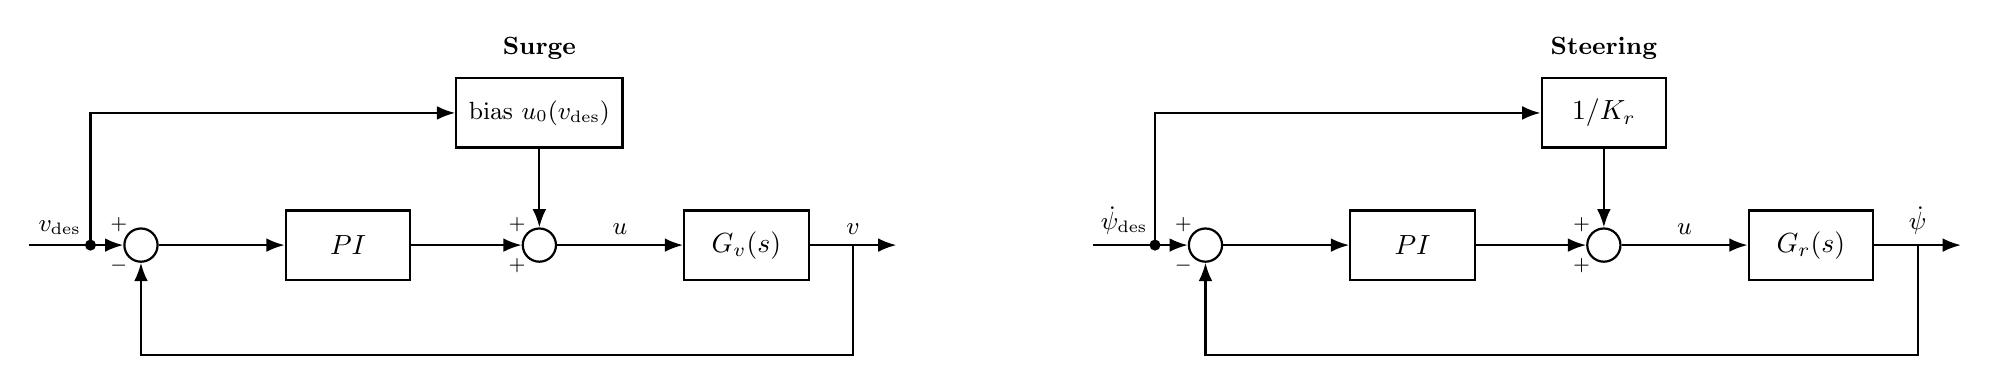
\begin{tikzpicture}[
  >=Latex, thick,
  block/.style = {draw, rectangle, minimum height=2.5em, minimum width=4.5em},
  sum/.style   = {draw, circle, inner sep=0pt, minimum size=1.2em},
]
%--- Left: Surge (operating-point bias) ---
  \node[coordinate]                              (srin)  {};
  \node[sum,   right=1.2cm of srin]             (ses)   {};
  \node[block, right=1.6cm of ses]              (sPI)   {$PI$};
  \node[sum,   right=1.4cm of sPI]              (sus)   {};
  \node[block, right=1.6cm of sus]              (sG)    {$G_v(s)$};
  \node[coordinate, right=1.1cm of sG]          (syo)   {};

  \node[block, above=1.0cm of sus, minimum width=6em]
                                                  (sbias) {\small bias $u_0(v_\text{des})$};

  \node[font=\small\bfseries, above=0.1cm of sbias] {Surge};

  \node[font=\scriptsize, inner sep=0pt, anchor=south east] at (ses.north west) {$+$};
  \node[font=\scriptsize, inner sep=0pt, anchor=north east] at (ses.south west) {$-$};
  \node[font=\scriptsize, inner sep=0pt, anchor=south east] at (sus.north west) {$+$};
  \node[font=\scriptsize, inner sep=0pt, anchor=north east] at (sus.south west) {$+$};

  \coordinate (srb) at ($(srin)!0.55!(ses)$);
  \draw    (srin) -- node[above,font=\small]{$v_\text{des}$} (srb);
  \draw[->] (srb) -- (ses);
  \fill (srb) circle (2pt);
  \draw[->] (srb)  |- (sbias);
  \draw[->] (sbias) -- (sus.north);
  \draw[->] (ses)  -- (sPI);
  \draw[->] (sPI)  -- (sus);
  \draw[->] (sus)  -- node[above,font=\small]{$u$} (sG);
  \draw[->] (sG)   -- node[above,font=\small]{$v$} (syo);

  \coordinate (sfbk) at ($(sG.east)!0.5!(syo)$);
  \draw[->] (sfbk) -- ++(0,-1.4) -| (ses.south);

%--- Right: Steering (proportional FF) ---
  \node[coordinate, right=2.5cm of syo]          (rrin)  {};
  \node[sum,   right=1.2cm of rrin]              (res)   {};
  \node[block, right=1.6cm of res]               (rPI)   {$PI$};
  \node[sum,   right=1.4cm of rPI]               (rus)   {};
  \node[block, right=1.6cm of rus]               (rG)    {$G_r(s)$};
  \node[coordinate, right=1.1cm of rG]           (ryo)   {};

  \node[block, above=1.0cm of rus]               (rFF)   {$1/K_r$};

  \node[font=\small\bfseries, above=0.1cm of rFF] {Steering};

  \node[font=\scriptsize, inner sep=0pt, anchor=south east] at (res.north west) {$+$};
  \node[font=\scriptsize, inner sep=0pt, anchor=north east] at (res.south west) {$-$};
  \node[font=\scriptsize, inner sep=0pt, anchor=south east] at (rus.north west) {$+$};
  \node[font=\scriptsize, inner sep=0pt, anchor=north east] at (rus.south west) {$+$};

  \coordinate (rrb) at ($(rrin)!0.55!(res)$);
  \draw    (rrin) -- node[above,font=\small]{$\dot\psi_\text{des}$} (rrb);
  \draw[->] (rrb) -- (res);
  \fill (rrb) circle (2pt);
  \draw[->] (rrb)  |- (rFF);
  \draw[->] (rFF)  -- (rus.north);
  \draw[->] (res)  -- (rPI);
  \draw[->] (rPI)  -- (rus);
  \draw[->] (rus)  -- node[above,font=\small]{$u$} (rG);
  \draw[->] (rG)   -- node[above,font=\small]{$\dot\psi$} (ryo);

  \coordinate (rfbk) at ($(rG.east)!0.5!(ryo)$);
  \draw[->] (rfbk) -- ++(0,-1.4) -| (res.south);
\end{tikzpicture}}
\caption{Feedforward configurations for surge (operating-point bias) and
  yaw-rate (proportional FF) control.}
\label{fig:ff_usv}
\end{figure}


% ===========================================================================
\section{Practical Modifications Beyond Ideal PID}
\label{sec:practical}
% ===========================================================================

The sections above developed the ideal PID controller.  Real implementations
modify this ideal in several important ways.  Because the lab asks you to
both simulate controllers in MATLAB and configure them on the vehicle, each
modification is discussed from two angles:

\begin{itemize}
  \item \textbf{Linear analysis (MATLAB):} how to represent the modification
    as a transfer function so it can be incorporated into a closed-loop model
    and analyzed with the tools from this course.
  \item \textbf{ArduRover implementation:} how the same idea is realized in
    the autopilot, which typically uses a discrete, nonlinear version.
\end{itemize}

The two approaches produce qualitatively similar behavior; the linear model
is an approximation that is useful for design and analysis, while the ArduRover
implementation handles the practical realities of a digital controller with
actuator limits.

% ---------------------------------------------------------------------------
\subsection{Anti-Windup}
% ---------------------------------------------------------------------------

\textbf{The problem.}  Every actuator has limits.  When the control output
saturates (throttle pinned at maximum, rudder at its mechanical stop), the
plant input is clipped to the saturation bound.  The integrator, however,
does not know this --- it keeps integrating the error as if the full output
were reaching the plant.  By the time the output leaves saturation, the
integrator has accumulated a value far beyond what is needed, causing a
large overshoot and slow recovery.  This is \emph{integral windup}.

\textbf{The fix: integrator clamping (ArduRover).}
The simplest anti-windup strategy stops integration whenever the output is
saturated and the error would push the integrator further in the saturating
direction.  Mathematically: if $u > u_\mathrm{max}$ and $e > 0$, freeze the
integral; if $u < u_\mathrm{min}$ and $e < 0$, freeze the integral.
Otherwise integrate normally.


In ArduRover, integral limits are enforced through output clamping in the PID
library; the \texttt{MOT\_SLEWRATE} parameter (discussed below) provides
complementary protection by preventing the output from changing so rapidly
that the plant saturates in the first place.

\textbf{The fix: back-calculation (linear analysis).}
Back-calculation is the anti-windup approach that lends itself to linear
modeling.  Rather than switching the integrator on and off (nonlinear), it
adds a continuous feedback path from the difference between the saturated
and unsaturated outputs back to the integrator input:
\begin{equation}
  \dot{x}_I = e(t) + \frac{1}{T_t}\bigl(u_\mathrm{sat} - u_\mathrm{raw}\bigr)
  \label{eq:backcalc}
\end{equation}
where $T_t$ is the \emph{tracking time constant} that sets how quickly the
integrator unwinds.  When the output is not saturated, $u_\mathrm{sat} =
u_\mathrm{raw}$ and the extra term vanishes --- the controller behaves as
normal.  When saturated, the feedback drives $\dot{x}_I$ toward zero,
preventing further wind-up.  A good starting point is $T_t = \sqrt{T_I T_D}$
(or simply $T_t = T_I$ for a PI controller).

The value of back-calculation for simulation is that the additional path
can be drawn in a Simulink or MATLAB block diagram and analyzed as part of
the linear loop structure.  It does not require a conditional logic block.

\begin{figure}[htbp]
\centering

\textbf{(a) Clamping}\\[0.4em]
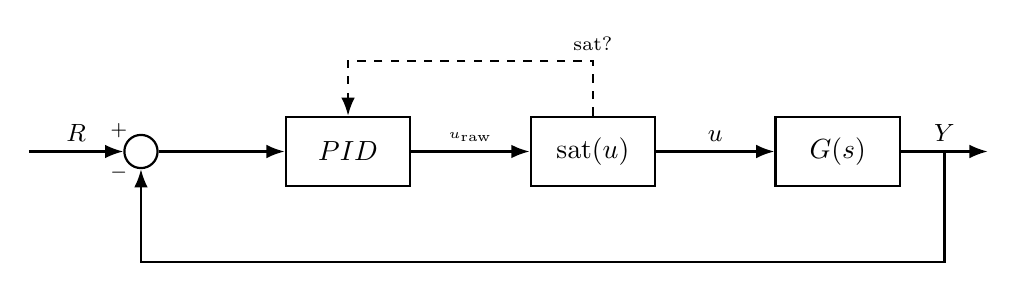
\begin{tikzpicture}[
  >=Latex, thick,
  block/.style = {draw, rectangle, minimum height=2.5em, minimum width=4.5em},
  sum/.style   = {draw, circle, inner sep=0pt, minimum size=1.2em},
]
  \node[coordinate]                                (arin)  {};
  \node[sum,   right=1.2cm of arin]                (aes)   {};
  \node[block, right=1.6cm of aes]                 (aPID)  {$PID$};
  \node[block, right=1.5cm of aPID,minimum width=4.5em] (asat) {sat$(u)$};
  \node[block, right=1.5cm of asat]                (aG)    {$G(s)$};
  \node[coordinate, right=1.1cm of aG]             (ayo)   {};

  \node[font=\scriptsize, inner sep=0pt, anchor=south east] at (aes.north west) {$+$};
  \node[font=\scriptsize, inner sep=0pt, anchor=north east] at (aes.south west) {$-$};

  \draw[->] (arin) -- node[above,font=\small]{$R$}          (aes);
  \draw[->] (aes)  --                                        (aPID);
  \draw[->] (aPID) -- node[above,font=\tiny]{$u_\mathrm{raw}$} (asat);
  \draw[->] (asat) -- node[above,font=\small]{$u$}           (aG);
  \draw[->] (aG)   -- node[above,font=\small]{$Y$}           (ayo);

  \coordinate (afbk) at ($(aG.east)!0.5!(ayo)$);
  \draw[->] (afbk) -- ++(0,-1.4) -| (aes.south);

  \draw[->,dashed] (asat.north) -- ++(0,0.7)
      node[above,font=\scriptsize]{sat?} -| (aPID.north);
\end{tikzpicture}

\bigskip
\textbf{(b) Back-calculation}\\[0.4em]
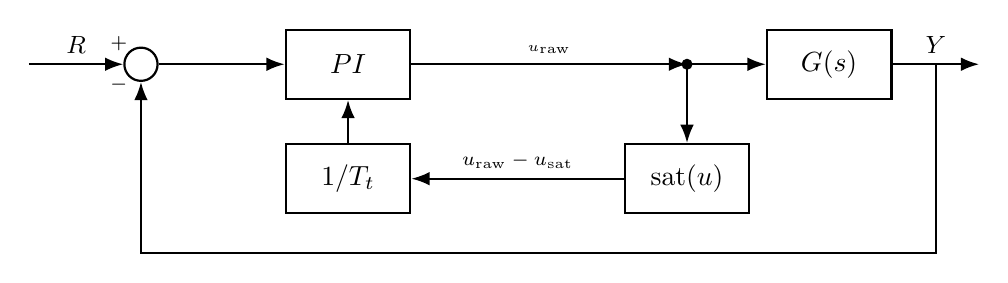
\begin{tikzpicture}[
  >=Latex, thick,
  block/.style = {draw, rectangle, minimum height=2.5em, minimum width=4.5em},
  sum/.style   = {draw, circle, inner sep=0pt, minimum size=1.2em},
]
  \node[coordinate]                                (brin)  {};
  \node[sum,   right=1.2cm of brin]                (bes)   {};
  \node[block, right=1.6cm of bes]                 (bPI)   {$PI$};
  % bus is a pickoff point, placed 3.5cm from bPI's right edge
  \coordinate (bus) at ($(bPI.east)+(3.5cm,0)$);
  \node[block, right=1.0cm of bus]                 (bG)    {$G(s)$};
  \node[coordinate, right=1.1cm of bG]             (byo)   {};

  \node[block, below=1.0cm of bus, minimum width=4.5em] (bsat) {sat$(u)$};
  % bTt aligned to same height as bsat but directly below bPI
  \node[block, minimum width=4.5em] (bTt) at (bPI |- bsat) {$1/T_t$};

  \node[font=\scriptsize, inner sep=0pt, anchor=south east] at (bes.north west) {$+$};
  \node[font=\scriptsize, inner sep=0pt, anchor=north east] at (bes.south west) {$-$};

  \draw[->] (brin) -- node[above,font=\small]{$R$}             (bes);
  \draw[->] (bes)  --                                           (bPI);
  \draw[->] (bPI)  -- node[above,font=\tiny]{$u_\mathrm{raw}$} (bus);
  \fill (bus) circle (2pt);
  \draw[->] (bus)  --                                           (bG);
  \draw[->] (bG)   -- node[above,font=\small]{$Y$}              (byo);

  \draw[->] (bus) -- (bsat.north);
  \draw[->] (bsat.west) -- node[above,font=\scriptsize]{$u_\mathrm{raw}-u_\mathrm{sat}$} (bTt.east);
  \draw[->] (bTt.north) -- (bPI.south);

  \coordinate (bfbk) at ($(bG.east)!0.5!(byo)$);
  \draw[->] (bfbk) -- ++(0,-2.4) -| (bes.south);
\end{tikzpicture}

\caption{Two anti-windup methods.  Clamping (a) is simpler to implement in
  code; back-calculation (b) can be represented as a linear feedback path
  for analysis.}
\label{fig:antiwindup_both}
\end{figure}

% ---------------------------------------------------------------------------
\subsection{Derivative on Measurement}
% ---------------------------------------------------------------------------

\textbf{The problem.}
When the reference $r(t)$ changes as a step, the error
$e(t) = r(t) - y(t)$ also steps instantaneously.  The derivative of a step
is an impulse --- so the D term briefly commands a very large (theoretically
infinite) actuator signal.  This \emph{derivative kick} is especially
disruptive for actuators like servos and propellers that can be damaged or
destabilized by impulsive commands.

\textbf{The fix.}
Compute the D term from the negative derivative of the \emph{measurement}
rather than the error:
\[
  u_D = -K_D\,\dot{y}
\]
Since the measurement changes smoothly (the plant cannot respond
instantaneously), $\dot{y}$ is well-behaved even when the reference steps.
The proportional and integral terms are still computed from $e = r - y$ as
usual.

\textbf{Example.}
Consider a speed controller with $K_D = 0.2$ and a setpoint step from 1~m/s
to 2~m/s at $t = 1$\,s.  With D on error: the error jumps from 0 to 1~m/s,
so $u_D$ spikes to $+0.2/\Delta t$ for one timestep (very large for a small
$\Delta t$).  With D on measurement: at $t = 1^+$, the measured speed is
still 1~m/s and $\dot{y} \approx 0$, so $u_D \approx 0$.  The derivative term
only activates as the speed actually begins to change --- which is exactly
when its damping action is needed.

\begin{figure}[htbp]
\centering
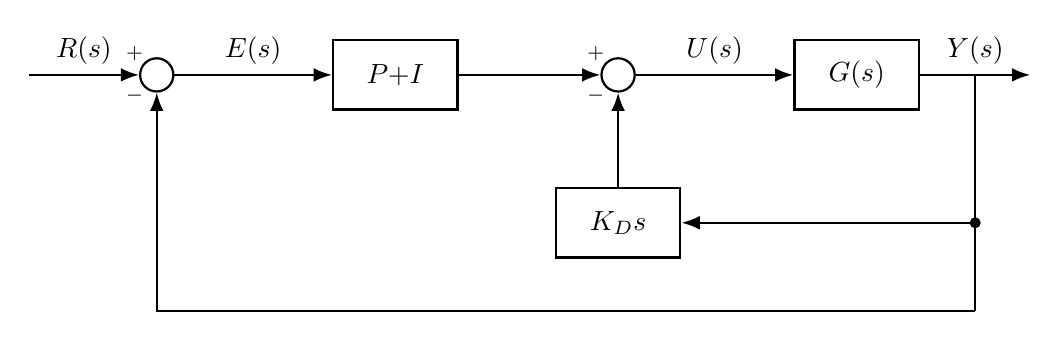
\begin{tikzpicture}[
  >=Latex, thick,
  block/.style = {draw, rectangle, minimum height=2.5em, minimum width=4.5em},
  sum/.style   = {draw, circle, inner sep=0pt, minimum size=1.2em},
]
  \node[coordinate]                    (rin)   {};
  \node[sum,   right=1.4cm of rin]     (esum)  {};
  \node[block, right=2.0cm of esum]    (PI)    {$P{+}I$};
  \node[sum,   right=1.8cm of PI]      (csum)  {};
  \node[block, right=2.0cm of csum]    (G)     {$G(s)$};
  \node[coordinate, right=1.4cm of G]  (yout)  {};

  % D block below csum, fed from output
  \node[block, below=1.2cm of csum]    (D)     {$K_D s$};

  \node[font=\scriptsize, inner sep=0pt, anchor=south east] at (esum.north west) {$+$};
  \node[font=\scriptsize, inner sep=0pt, anchor=north east] at (esum.south west) {$-$};
  \node[font=\scriptsize, inner sep=0pt, anchor=south east] at (csum.north west) {$+$};
  \node[font=\scriptsize, inner sep=0pt, anchor=north east] at (csum.south west) {$-$};

  \draw[->] (rin)   -- node[above]{$R(s)$} (esum);
  \draw[->] (esum)  -- node[above]{$E(s)$} (PI);
  \draw[->] (PI)    -- node[above]{}        (csum);
  \draw[->] (csum)  -- node[above]{$U(s)$} (G);
  \draw[->] (G)     -- node[above]{$Y(s)$} (yout);

  % feedback to esum; wire goes deep enough to clear D block below
  \coordinate (fbk) at ($(G.east)!0.5!(yout)$);
  \draw (fbk) -- ++(0,-3.0);
  \coordinate (fbot) at ($(fbk)+(0,-3.0)$);
  \draw[->] (fbot) -| (esum.south);

  % D path: branch from feedback wire at D's height, straight horizontal to D.east
  \coordinate (dbranch) at (fbk |- D.east);
  \fill (dbranch) circle (2pt);
  \draw[->] (dbranch) -- (D.east);
  \draw[->] (D.north) -- (csum.south);
\end{tikzpicture}
\caption{Derivative on measurement: the D term is computed from $-\dot{y}$
  rather than $\dot{e}$, eliminating derivative kick on setpoint steps.}
\label{fig:d_on_meas}
\end{figure}

% ---------------------------------------------------------------------------
\subsection{Derivative Filtering}
% ---------------------------------------------------------------------------

\textbf{The problem.}
Even with the derivative computed on the measurement, high-frequency noise in
the sensor signal causes problems.  The D term amplifies rapid changes, and
sensor noise consists of exactly those rapid, small fluctuations.  The result
is large, fast actuator oscillations that wear out hardware and destabilize
the plant.

\textbf{The fix.}
Add a first-order lag in series with the differentiator:
\begin{equation}
  D_f(s) = \frac{K_D s}{\tau_f s + 1}
  \label{eq:d_filtered}
\end{equation}

To understand what this does, consider two extremes.  For slowly varying
signals (small $s$), the denominator $\tau_f s + 1 \approx 1$, and $D_f(s)
\approx K_D s$ --- pure differentiation, as intended.  For rapidly varying
signals (large $s$), the denominator dominates: $D_f(s) \approx K_D/\tau_f$,
a constant gain.  The D term no longer amplifies noise without bound; its gain
is capped at $K_D/\tau_f$ for rapid changes.

The parameter $\tau_f$ is a tuning knob.  A small $\tau_f$ passes high
frequencies more readily --- the D term is more responsive but also noisier.
A large $\tau_f$ filters aggressively but blunts the D term's effectiveness
at the frequencies of interest.  In practice, $\tau_f$ is often set to
$K_D/(5\text{ to }10)$ as a starting point.

\textbf{Linear analysis (MATLAB).}
The filtered PID transfer function is:
\begin{equation}
  C_f(s) = K_P + \frac{K_I}{s} + \frac{K_D s}{\tau_f s + 1}
  \label{eq:pid_filtered_tf}
\end{equation}
This is a proper, rational transfer function that can be entered directly
into MATLAB and used in any closed-loop analysis.  When you cover frequency
response later in the course, \cref{eq:d_filtered} will look familiar as a
\emph{lead compensator} --- a device that adds phase lead while bounding
its high-frequency gain.

\textbf{ArduRover implementation.}
ArduRover applies an exponential moving average (EMA) to the derivative
measurement at each timestep, which is the discrete-time equivalent of the
first-order lag in \cref{eq:d_filtered}.

\begin{figure}[htbp]
\centering
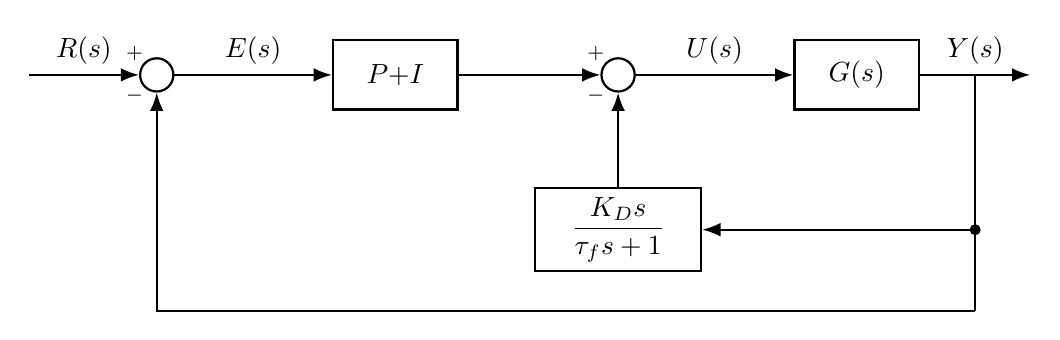
\begin{tikzpicture}[
  >=Latex, thick,
  block/.style = {draw, rectangle, minimum height=2.5em, minimum width=4.5em},
  sum/.style   = {draw, circle, inner sep=0pt, minimum size=1.2em},
]
  \node[coordinate]                    (rin)   {};
  \node[sum,   right=1.4cm of rin]     (esum)  {};
  \node[block, right=2.0cm of esum]    (PI)    {$P{+}I$};
  \node[sum,   right=1.8cm of PI]      (csum)  {};
  \node[block, right=2.0cm of csum]    (G)     {$G(s)$};
  \node[coordinate, right=1.4cm of G]  (yout)  {};

  % filtered D block below csum
  \node[block, below=1.2cm of csum, minimum width=6em]
                                        (D)    {$\dfrac{K_D s}{\tau_f s+1}$};

  \node[font=\scriptsize, inner sep=0pt, anchor=south east] at (esum.north west) {$+$};
  \node[font=\scriptsize, inner sep=0pt, anchor=north east] at (esum.south west) {$-$};
  \node[font=\scriptsize, inner sep=0pt, anchor=south east] at (csum.north west) {$+$};
  \node[font=\scriptsize, inner sep=0pt, anchor=north east] at (csum.south west) {$-$};

  \draw[->] (rin)   -- node[above]{$R(s)$} (esum);
  \draw[->] (esum)  -- node[above]{$E(s)$} (PI);
  \draw[->] (PI)    --                      (csum);
  \draw[->] (csum)  -- node[above]{$U(s)$} (G);
  \draw[->] (G)     -- node[above]{$Y(s)$} (yout);

  \coordinate (fbk) at ($(G.east)!0.5!(yout)$);
  \draw (fbk) -- ++(0,-3.0);
  \coordinate (fbot) at ($(fbk)+(0,-3.0)$);
  \draw[->] (fbot) -| (esum.south);

  \coordinate (dbranch) at (fbk |- D.east);
  \fill (dbranch) circle (2pt);
  \draw[->] (dbranch) -- (D.east);
  \draw[->] (D.north) -- (csum.south);
\end{tikzpicture}
\caption{Filtered derivative: the first-order lag caps the D term gain at
  high frequencies, reducing noise amplification.}
\label{fig:d_filtered}
\end{figure}



% ---------------------------------------------------------------------------
\subsection{Output Slew Rate Limiting}
% ---------------------------------------------------------------------------

\textbf{The problem.}
Very rapid changes in controller output can excite dynamics that the PID
model ignores: propeller cavitation, mechanical resonance in drive shafts,
or current spikes that drain batteries and trigger overcurrent faults.
A PID controller with high gains can, in principle, command the actuator to
jump from one extreme to the other in a single timestep.

\textbf{The fix (ArduRover).}
Limit the rate at which the controller output is allowed to change.  If the
desired output $u_\mathrm{raw}$ would require a change larger than
$S_\mathrm{max}\,\Delta t$ from the previous output, clamp it:
\begin{equation}
  u = u_\mathrm{prev} + \mathrm{clamp}\!\left(\,u_\mathrm{raw} - u_\mathrm{prev},\;
      -S_\mathrm{max}\Delta t,\; +S_\mathrm{max}\Delta t\right)
\end{equation}

This does not reduce the ultimate steady-state value the output reaches; it
only limits how quickly it gets there.

\begin{figure}[htbp]
\centering
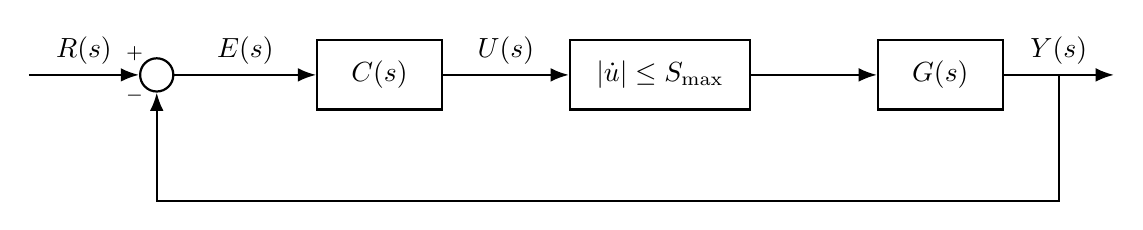
\begin{tikzpicture}[
  >=Latex, thick,
  block/.style = {draw, rectangle, minimum height=2.5em, minimum width=4.5em},
  sum/.style   = {draw, circle, inner sep=0pt, minimum size=1.2em},
]
  \node[coordinate]                                    (rin)  {};
  \node[sum,   right=1.4cm of rin]                     (sum)  {};
  \node[block, right=1.8cm of sum]                     (C)    {$C(s)$};
  \node[block, right=1.6cm of C, minimum width=6.5em]  (slew) {$|\dot{u}| \leq S_\mathrm{max}$};
  \node[block, right=1.6cm of slew]                    (G)    {$G(s)$};
  \node[coordinate, right=1.4cm of G]                  (yout) {};

  \node[font=\scriptsize, inner sep=0pt, anchor=south east] at (sum.north west) {$+$};
  \node[font=\scriptsize, inner sep=0pt, anchor=north east] at (sum.south west) {$-$};

  \draw[->] (rin)  -- node[above]{$R(s)$}  (sum);
  \draw[->] (sum)  -- node[above]{$E(s)$}  (C);
  \draw[->] (C)    -- node[above]{$U(s)$}  (slew);
  \draw[->] (slew) --                       (G);
  \draw[->] (G)    -- node[above]{$Y(s)$}  (yout);

  \coordinate (fbk) at ($(G.east)!0.5!(yout)$);
  \draw[->] (fbk) -- ++(0,-1.6) -| (sum.south);
\end{tikzpicture}
\caption{Slew rate limiter placed between the controller and the plant.}
\label{fig:slewrate}
\end{figure}


In ArduRover, \texttt{MOT\_SLEWRATE} sets the maximum throttle change rate
(units: fraction per second on a 0--100 scale).  Setting it to zero disables
slew limiting entirely.

\textbf{Linear analysis (MATLAB).}
A slew rate limiter is nonlinear, but for small signals (where the rate limit
is not active) it behaves like a unity gain.  For linear analysis, a
first-order lag on the controller output is a tractable approximation:
\begin{equation}
  U_\mathrm{plant}(s) = \frac{1}{\tau_s s + 1}\,U_\mathrm{raw}(s)
  \label{eq:slewrate_linear}
\end{equation}
Choose $\tau_s$ to reflect the effective smoothing: if the slew rate is
$S_\mathrm{max}$ (units/s) and the full actuator range is $\Delta u$, then
$\tau_s \approx \Delta u / (2 S_\mathrm{max})$ is a reasonable estimate.
This first-order lag adds a pole to the open-loop transfer function and can
reduce the phase margin --- an important check when tuning aggressive gains.

% ---------------------------------------------------------------------------
\subsection{Setpoint Prefiltering and Trajectory Constraints}
% ---------------------------------------------------------------------------

\textbf{The problem.}
Step changes in the reference signal are a useful tool for system
identification and testing --- a sudden speed or heading command reveals the
plant dynamics cleanly.  In operation, however, commanding an instantaneous
jump in speed asks the vehicle to produce infinite acceleration: physically
impossible, and a guarantee that the actuator will saturate and the integrator
will wind up before the plant can begin to respond.

More broadly, there is a mismatch between what the \emph{controller} asks for
(instantaneous change) and what the \emph{plant} can deliver (bounded
acceleration).  Driving the controller hard against a limit it cannot
satisfy activates dynamics that are harder to control --- saturated actuators,
windup, and sharp transients that can excite structural resonances.

\textbf{The fix.}
The problem is not in the feedback loop but in the reference signal.  Replace
the step command with a smoothed reference that changes at a rate the vehicle
can actually achieve.  For speed control, $a_\mathrm{max}$ is literally an
acceleration limit (m/s$^2$): the commanded speed ramps up at no more than
$a_\mathrm{max}$ meters per second per second.  For heading, it is a turning
rate limit.  This is not a modification to the PID controller itself, but to
the signal that feeds it.

Two standard implementations exist, and they produce qualitatively similar
results with different shapes:

\textbf{Linear analysis (MATLAB) --- first-order reference filter.}
A first-order low-pass filter on the reference is the linear option:
\begin{equation}
  R_f(s) = \frac{1}{\tau_r s + 1}\,R(s)
  \label{eq:reffilter}
\end{equation}
For a step in $R$, the filtered reference $R_f$ rises exponentially with
time constant $\tau_r$ rather than instantaneously.  This can be added to
the front of any MATLAB transfer function model, and the overall closed-loop
from $R$ to $Y$ becomes $T(s)/(\tau_r s + 1)$.  Choose $\tau_r$ to keep
the demanded acceleration within the vehicle's capability.

\textbf{ArduRover --- rate limiter.}
A rate limiter converts a step command into a ramp: the reference increases
linearly at $a_\mathrm{max}$ until it reaches the new setpoint, then holds.
This is nonlinear (the output slope is capped regardless of how large the
step is) but provides a hard, predictable bound on the demanded acceleration.
The shapes differ: the low-pass filter gives an exponentially decelerating
approach, while the rate limiter gives a constant-rate ramp followed by
a sharp corner.  For analysis, the low-pass filter is the better model; for
deployment, ArduRover's rate limiter provides more predictable actuator
loading.

\begin{figure}[htbp]
\centering
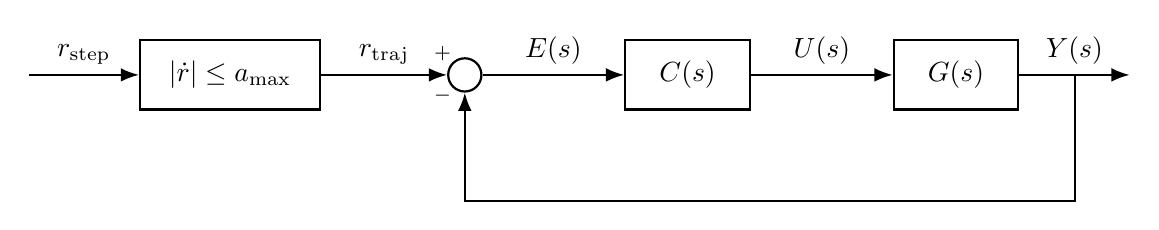
\begin{tikzpicture}[
  >=Latex, thick,
  block/.style = {draw, rectangle, minimum height=2.5em, minimum width=4.5em},
  sum/.style   = {draw, circle, inner sep=0pt, minimum size=1.2em},
]
  \node[coordinate]                                      (rin)    {};
  \node[block, right=1.4cm of rin, minimum width=6.5em]  (filt)   {$|\dot{r}| \leq a_\mathrm{max}$};
  \node[sum,   right=1.6cm of filt]                      (sum)    {};
  \node[block, right=1.8cm of sum]                       (C)      {$C(s)$};
  \node[block, right=1.8cm of C]                         (G)      {$G(s)$};
  \node[coordinate, right=1.4cm of G]                    (yout)   {};

  \node[font=\scriptsize, inner sep=0pt, anchor=south east] at (sum.north west) {$+$};
  \node[font=\scriptsize, inner sep=0pt, anchor=north east] at (sum.south west) {$-$};

  \draw[->] (rin)   -- node[above]{$r_\mathrm{step}$}   (filt);
  \draw[->] (filt)  -- node[above]{$r_\mathrm{traj}$}   (sum);
  \draw[->] (sum)   -- node[above]{$E(s)$}              (C);
  \draw[->] (C)     -- node[above]{$U(s)$}              (G);
  \draw[->] (G)     -- node[above]{$Y(s)$}              (yout);

  \coordinate (fbk) at ($(G.east)!0.5!(yout)$);
  \draw[->] (fbk) -- ++(0,-1.6) -| (sum.south);
\end{tikzpicture}
\caption{Setpoint prefilter: a rate limiter on the reference prevents the
  controller from being driven against actuator limits.}
\label{fig:prefilter}
\end{figure}

In ArduRover, \texttt{ATC\_ACCEL\_MAX} and \texttt{ATC\_DECEL\_MAX} set the
maximum acceleration and deceleration rates for the speed command.  Setting
asymmetric values (e.g., slower deceleration limit for a vehicle with weak
braking) is a natural extension of the rate-limiter concept.


% ===========================================================================
\section{Tuning Methods}
\label{sec:tuning}
% ===========================================================================

\subsection{Two Categories of Parameters}
\label{sec:two_categories}

Before selecting any gains, it helps to recognise that the ArduRover speed
controller has two fundamentally different kinds of tunable parameters.

\textbf{Category 1 — Set from system knowledge.}  These parameters have
correct values that can be determined analytically or read directly from
hardware specifications, without iteration on the vehicle:
\begin{itemize}
  \item \emph{Input filter cutoffs} (\texttt{\_FLTT}, acceleration limit):
    matched to the desired reference bandwidth and vehicle performance limits.
  \item \emph{Error and derivative filter cutoffs} (\texttt{\_FLTE},
    \texttt{\_FLTD}): chosen from sensor noise characteristics (sample rate,
    noise floor).
  \item \emph{Anti-windup limit} (\texttt{\_IMAX}): set to the actuator
    saturation bound, which is a known hardware property.
  \item \emph{Baseline feedforward} (\texttt{throttle baseline} or
    \texttt{\_FF}): the linearised steady-state throttle required to hold
    cruise speed, derivable from the plant DC gain $K_v$.  Use one or the
    other; they are redundant.
  \item \emph{Derivative feedforward} (\texttt{\_DFF}): initial value
    from the plant model; refined in field testing.
\end{itemize}

\textbf{Category 2 — Gains tuned iteratively.}  These cannot be set
analytically without a precise nonlinear model, and are best found by
simulation first, then refined on the vehicle:
\begin{itemize}
  \item Proportional, integral, and derivative gains
    ($K_P$, $K_I$, $K_D$ — \texttt{\_P}, \texttt{\_I}, \texttt{\_D}).
\end{itemize}

\subsection{Linear Transfer Function Model}
\label{sec:tf_model}

Simulation against the linear plant model allows
Category~2 gains to be explored safely before going to the water.
\Cref{fig:speed_loop_linear} shows the full speed controller recast as
a block diagram of transfer functions; all nonlinear elements are linearised
as noted in \cref{tab:linearisations}.

\begin{table}[htbp]
\centering
\caption{Linearisation of nonlinear ArduRover elements for simulation.}
\label{tab:linearisations}
\begin{tabular}{lll}
\toprule
Element & Nonlinearity & Linear approximation \\
\midrule
Acceleration limit & Rate limiter   & First-order low-pass $\omega_a/(s+\omega_a)$ \\
Throttle baseline  & Lookup table   & Gain $K_{base}$ (slope at operating point) \\
Anti-windup \texttt{\_IMAX} & Saturation & Omitted (assume unsaturated) \\
Dmod / PD scale    & Slew limiter $\times$ gain & Combined gain $K_{pd}$ \\
\bottomrule
\end{tabular}
\end{table}

\begin{figure}[htbp]
\centering
\resizebox{\linewidth}{!}{%
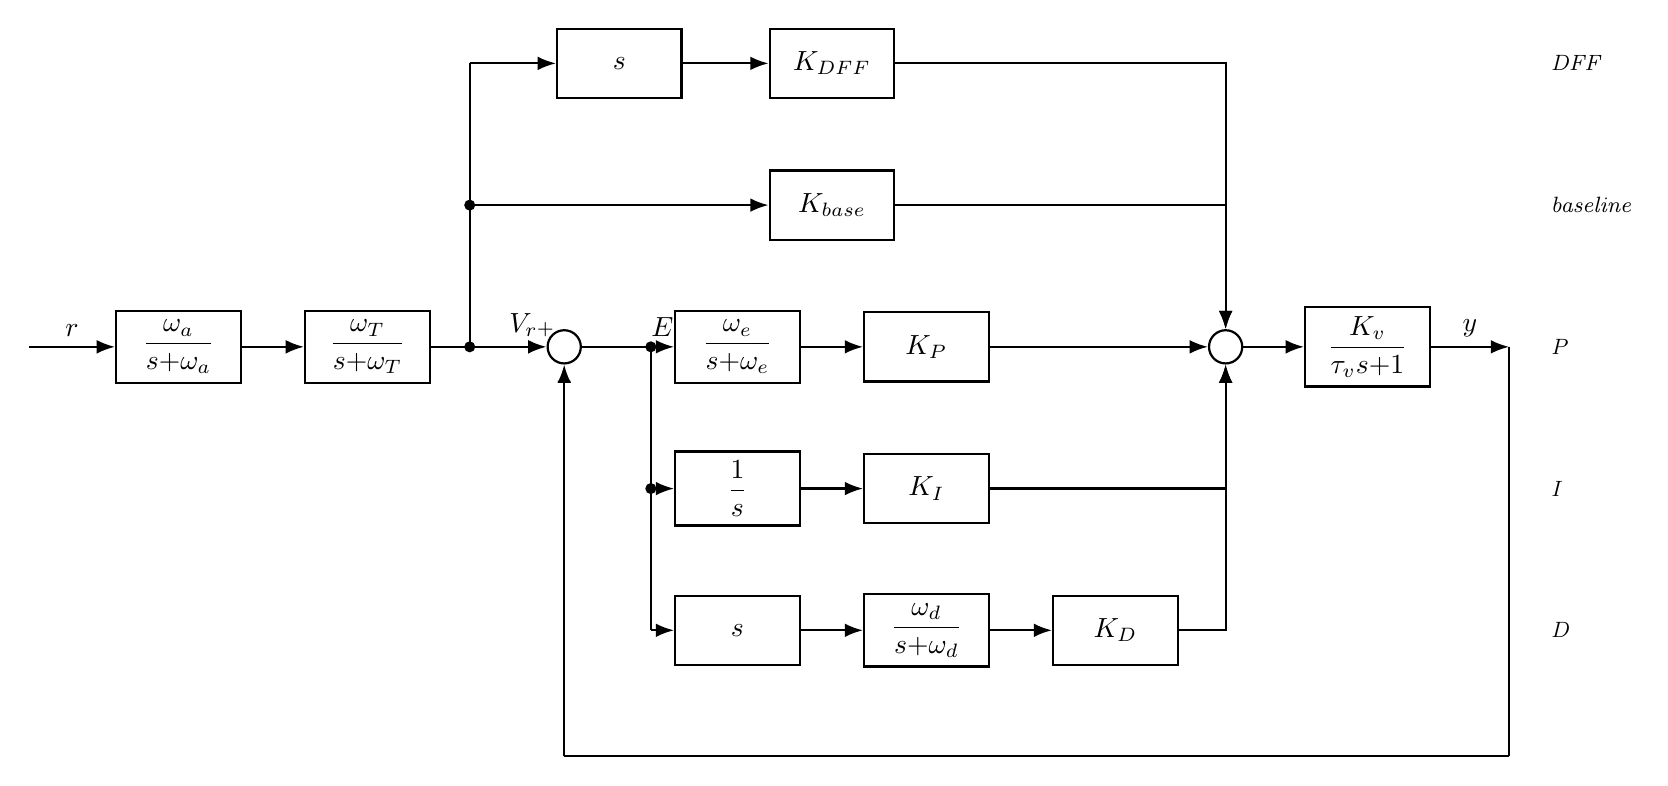
\begin{tikzpicture}[
  >=Latex, thick,
  block/.style = {draw, rectangle, minimum height=2.5em, minimum width=4.5em, align=center},
  sum/.style   = {draw, circle, inner sep=0pt, minimum size=1.2em},
]

%── Nodes ─────────────────────────────────────────────────────────────────────
% Main / P row (y = 0)
\node[coordinate]   (rin)  at (0,    0) {};
\node[block]        (facc) at (1.9,  0) {$\dfrac{\omega_a}{s{+}\omega_a}$};
\node[block]        (fltt) at (4.3,  0) {$\dfrac{\omega_T}{s{+}\omega_T}$};
\node[sum]          (esum) at (6.8,  0) {};
\node[block]        (flte) at (9.0,  0) {$\dfrac{\omega_e}{s{+}\omega_e}$};
\node[block]        (kp)   at (11.4, 0) {$K_P$};
\node[sum]          (osum) at (15.2, 0) {};
\node[block]        (gv)   at (17.0, 0) {$\dfrac{K_v}{\tau_v s{+}1}$};
\node[coordinate]   (yout) at (18.8, 0) {};

% DFF row (y = +3.6)
\node[block]        (sdff) at (7.5,  3.6) {$s$};
\node[block]        (kdff) at (10.2, 3.6) {$K_{DFF}$};

% Baseline row (y = +1.8)
\node[block]        (kbase)at (10.2, 1.8) {$K_{base}$};

% I row (y = −1.8)
\node[block]        (integ)at (9.0, -1.8) {$\dfrac{1}{s}$};
\node[block]        (ki)   at (11.4,-1.8) {$K_I$};

% D row (y = −3.6)
\node[block]        (sdiff)at (9.0, -3.6) {$s$};
\node[block]        (fltd) at (11.4,-3.6) {$\dfrac{\omega_d}{s{+}\omega_d}$};
\node[block]        (kd)   at (13.8,-3.6) {$K_D$};

%── Pickup coordinates ────────────────────────────────────────────────────────
\coordinate (vr)    at (5.6,  0);     % V_r: between fltt and esum
\coordinate (vr18)  at (5.6,  1.8);   % V_r spine at FF row
\coordinate (vr36)  at (5.6,  3.6);   % V_r spine at DFF row
\coordinate (ebus)  at (7.9,  0);     % error bus: between esum and flte
\coordinate (ebus18)at (7.9, -1.8);   % error spine at I row
\coordinate (ebus36)at (7.9, -3.6);   % error spine at D row

%── Main row wires ────────────────────────────────────────────────────────────
\draw[->] (rin)       -- node[above]{$r$}          (facc.west);
\draw[->] (facc)      --                            (fltt.west);
\draw     (fltt.east) --                            (vr);
\draw[->] (vr)        -- node[above,pos=0.7]{$V_r$}(esum.west);
\draw     (esum.east) --                            (ebus);
\draw[->] (ebus)      -- node[above,pos=0.5]{$E$}  (flte.west);
\draw[->] (flte)      --                            (kp.west);
\draw[->] (kp.east)   --                            (osum.west);
\draw[->] (osum)      --                            (gv.west);
\draw[->] (gv.east)   -- node[above]{$y$}           (yout);

%── Sum sign labels ───────────────────────────────────────────────────────────
\node[above left, font=\scriptsize]  at (esum) {$+$};
\node[below,      font=\scriptsize]  at (esum.south) {$-$};

%── Pickoff dots ──────────────────────────────────────────────────────────────
\fill (vr)    circle (2pt);
\fill (vr18)  circle (2pt);
\fill (ebus)  circle (2pt);
\fill (ebus18)circle (2pt);

%── V_r vertical spine ────────────────────────────────────────────────────────
\draw (vr) -- (vr18) -- (vr36);

%── Baseline path: vr18 → kbase → osum ───────────────────────────────────────
\draw[->] (vr18)       --                           (kbase.west);
\draw[->] (kbase.east) -- (kbase.east -| osum)  --  (osum.north);

%── DFF path: vr36 → sdff → kdff → osum ──────────────────────────────────────
\draw[->] (vr36)       --                           (sdff.west);
\draw[->] (sdff)       --                           (kdff.west);
\draw[->] (kdff.east)  -- (kdff.east  -| osum)  --  (osum.north);

%── Error vertical spine ──────────────────────────────────────────────────────
\draw (ebus) -- (ebus18) -- (ebus36);

%── I path: ebus18 → integ → ki → osum ───────────────────────────────────────
\draw[->] (ebus18)     --                           (integ.west);
\draw[->] (integ)      --                           (ki.west);
\draw[->] (ki.east)    -- (ki.east    -| osum)  --  (osum.south);

%── D path: ebus36 → sdiff → fltd → kd → osum ────────────────────────────────
\draw[->] (ebus36)     --                           (sdiff.west);
\draw[->] (sdiff)      --                           (fltd.west);
\draw[->] (fltd)       --                           (kd.west);
\draw[->] (kd.east)    -- (kd.east    -| osum)  --  (osum.south);

%── Feedback wire: yout → below → esum.south ─────────────────────────────────
\draw     (yout)       -- ++(0,-5.2);
\draw     ($(yout)+(0,-5.2)$) -- ($(esum)+(0,-5.2)$);
\draw[->] ($(esum)+(0,-5.2)$) --  (esum.south);

%── Row labels (right margin) ─────────────────────────────────────────────────
\node[right, font=\footnotesize\itshape] at (19.2,  3.6) {DFF};
\node[right, font=\footnotesize\itshape] at (19.2,  1.8) {baseline};
\node[right, font=\footnotesize\itshape] at (19.2,  0)   {P};
\node[right, font=\footnotesize\itshape] at (19.2, -1.8) {I};
\node[right, font=\footnotesize\itshape] at (19.2, -3.6) {D};

\end{tikzpicture}%
}
\caption{Linear transfer function model of the ArduRover speed controller.
  Input shaping: $\omega_a/(s{+}\omega_a)$ (acceleration limit) and
  $\omega_T/(s{+}\omega_T)$ (\texttt{\_FLTT}) produce the filtered reference
  $V_r$.  Feedforward paths act on $V_r$ directly; feedback paths act on
  the error $E = V_r - y$.  The error filter $\omega_e/(s{+}\omega_e)$
  (\texttt{\_FLTE}) applies only to the P path; the D-term filter
  $\omega_d/(s{+}\omega_d)$ (\texttt{\_FLTD}) attenuates derivative noise.
  Nonlinear elements are linearised per \cref{tab:linearisations}.
  The companion script \texttt{sim\_speed\_loop.m} implements this model
  in MATLAB for closed-loop simulation.}
\label{fig:speed_loop_linear}
\end{figure}

\begin{table}[htbp]
\centering
\caption{Filter and input-shaping parameters of the linear speed-loop model.
  ArduRover parameter names are shown where applicable.
  Recommended values are starting points; the plant time constant $\tau_v$
  comes from system identification.}
\label{tab:filter_params}
\begin{tabular}{llp{4.8cm}l}
\toprule
Symbol & ArduRover param. & Description & Recommended start \\
\midrule
$\tau_v$ & --- (plant) &
  Surge time constant identified from sea trials &
  $\approx 1.5$~s (identified) \\
$\omega_a$ & \texttt{ATC\_ACCEL\_MAX} &
  First-order approximation of the trajectory acceleration limiter
  ($\omega_a = a_{\max}/v_{\rm cruise}$) &
  $1$--$2$~rad/s \\
$\omega_T$ & \texttt{\_FLTT} &
  Low-pass filter on the target (reference) speed &
  $1/\tau_v$--$2/\tau_v$~rad/s \\
$\omega_e$ & \texttt{\_FLTE} &
  Low-pass filter on the speed error (P path only) &
  $3$--$5\,\omega_T$ \\
$\omega_d$ & \texttt{\_FLTD} &
  Low-pass filter on the derivative term (noise rejection) &
  $5$--$10\,\omega_T$ \\
\bottomrule
\end{tabular}
\end{table}

\subsection{The Case for Intuition First}

The sections above built the tools to answer a diagnostic question: given a
poorly performing step response, which gain should change and in which
direction?  Flat steady-state error with a well-behaved transient: increase
$K_I$ or add integral.  Fast oscillations that don't decay: reduce $K_P$ or
$K_I$.  Slow convergence with no oscillation: increase $K_P$.  Overshoot that
takes many cycles to settle: reduce $K_I$ or add $K_D$.

Good intuition makes systematic gain selection possible.  The process below
uses the identified plant model in MATLAB simulation, so mistakes are free.
  
\subsection{A Systematic Tuning Process}

\begin{enumerate}
  \item \textbf{Start in simulation.}  Build the closed-loop model in MATLAB
    using the identified transfer functions.  All gain
    choices should be validated here before touching the vehicle.

  \item \textbf{P only first.}  Set $K_I = 0$ and $K_D = 0$.  Increase
    $K_P$ until the step response is fast with modest overshoot.  Note the
    remaining steady-state error; the next step removes it.

  \item \textbf{Add integral conservatively.}  Use \cref{eq:pi_params} with
    a modest target $\omega_n$, then choose $K_P$ for $\zeta \approx 0.7$.
    Verify the response has no more overshoot than the P-only case.
    Keep $K_I < K_P$.

  \item \textbf{Add derivative only if needed.}  For a first-order plant
    with PI, this is often unnecessary.  If the PI response is too
    oscillatory and increasing $K_P$ does not help, add a small $K_D$.

  \item \textbf{Verify disturbance rejection.}  Apply a step disturbance
    (simulated current or wind gust) and confirm recovery is acceptable.

  \item \textbf{Transfer to the vehicle cautiously.}  Start at roughly half
    the simulation gains, then increase in small steps while watching the
    actual response.
\end{enumerate}

\subsection{Troubleshooting by Symptom}

\Cref{tab:troubleshoot} maps observable step-response symptoms to causes and
corrective actions.

\begin{table}[htbp]
\centering
\caption{PID troubleshooting guide.}
\label{tab:troubleshoot}
\begin{tabular}{p{4cm}p{3.5cm}p{5cm}}
\toprule
Symptom & Likely cause & Action \\
\midrule
Nonzero steady-state error, clean transient
  & $K_I = 0$ or too small
  & Add or increase $K_I$; check anti-windup is not blocking integration \\[4pt]
Slow rise, sluggish response
  & $K_P$ too small
  & Increase $K_P$ \\[4pt]
Sustained oscillation
  & $K_P$ or $K_I$ too large
  & Reduce $K_I$ first; then $K_P$ if still oscillating \\[4pt]
Overshoot with slow settling
  & $K_I$ too large
  & Reduce $K_I$; consider adding $K_D$ for damping \\[4pt]
Large overshoot on large steps
  & Integral windup during saturation
  & Enable anti-windup; add setpoint prefilter \\[4pt]
Noisy or chattering actuator
  & $K_D$ too large or unfiltered
  & Reduce $K_D$; increase $\tau_f$ in derivative filter \\[4pt]
Actuator spike on setpoint step
  & Derivative kick
  & Switch to derivative on measurement \\[4pt]
Sluggish heading despite fast yaw rate
  & Inner loop too slow
  & Retune inner loop; reduce $\tau_\mathrm{cl}$ \\
\bottomrule
\end{tabular}
\end{table}


% ===========================================================================
\section{Summary}
\label{sec:summary}
% ===========================================================================

PID control is most useful when understood as a design progression, not a
collection of independent tricks.  Proportional control provides fast response
but leaves steady-state error.  Integral action eliminates that error by
accumulating history, at the cost of potential windup and oscillation if
$K_I$ is too large.  Derivative action adds damping --- most valuable when the
plant's natural dynamics provide little of it.

Heading control on the USV illustrates that the choice of loop architecture
matters as much as the choice of gains.  A single feedback loop around the
kinematic heading plant couples speed and damping in a way that limits
performance; cascade control separates the problem into two well-posed
first-order loops that can be tuned independently.

Feedforward shifts some of the burden from feedback to prediction.  An
operating-point bias handles the known, steady disturbance of drag at cruise;
proportional feedforward handles continuously varying yaw-rate commands.  In
both cases, the feedback loop is left to handle what feedforward cannot: model
error and disturbances.

The practical modifications in \cref{sec:practical} are not edge cases --- they
are standard features of production controllers, and ArduRover implements each
of them.  Understanding why each modification exists is the difference between
a controller that works in a lab and one that works on the water.

\Cref{tab:summary} maps the concepts developed in this article to their
ArduRover counterparts.

\begin{table}[htbp]
\centering
\caption{Concept-to-parameter mapping for ArduRover speed and steering control.}
\label{tab:summary}
\begin{tabular}{lll}
\toprule
Concept & ArduRover Parameter & Section \\
\midrule
Proportional gain (speed)    & \texttt{ATC\_SPEED\_P}                             & \cref{sec:pcontrol} \\
Proportional gain (steering) & \texttt{ATC\_STR\_RAT\_P}                          & \cref{sec:pcontrol} \\
Integral gain (speed)        & \texttt{ATC\_SPEED\_I}                             & \cref{sec:integral} \\
Integral gain (steering)     & \texttt{ATC\_STR\_RAT\_I}                          & \cref{sec:integral} \\
Derivative gain (speed)      & \texttt{ATC\_SPEED\_D}                             & \cref{sec:derivative} \\
Derivative gain (steering)   & \texttt{ATC\_STR\_RAT\_D}                          & \cref{sec:derivative} \\
Operating-point feedforward  & \texttt{CRUISE\_THROTTLE}, \texttt{CRUISE\_SPEED}  & \cref{sec:feedforward} \\
Proportional feedforward     & \texttt{ATC\_STR\_RAT\_FF}                         & \cref{sec:feedforward} \\
Anti-windup                  & Output clamping (internal)                         & \cref{sec:practical} \\
Output slew rate limit       & \texttt{MOT\_SLEWRATE}                             & \cref{sec:practical} \\
Trajectory constraint        & \texttt{ATC\_ACCEL\_MAX}, \texttt{ATC\_DECEL\_MAX} & \cref{sec:practical} \\
Cascade inner loop           & \texttt{ATC\_STR\_RAT\_*}                          & \cref{sec:cascade} \\
Cascade outer loop           & Navigation controller                              & \cref{sec:cascade} \\
\bottomrule
\end{tabular}
\end{table}

\end{document}
